\documentclass{bioinfo}
\copyrightyear{2019}
\pubyear{2019}
\usepackage{listings}
\usepackage{multicol}
\begin{document}
\firstpage{1}

\title[Microarray Analysis of miRNAs]{A Computational Model for the Early Detection of Primary Breast Cancer Using Differential Expression Analysis of Microarray Data from Serum microRNA}
\author[Krishna \textit{Sudhir}]{Krishna Sudhir\footnote{sudhir20k@ncssm.edu}}

\history{Submitted on 05/28/2019}
\maketitle

\begin{abstract}

Breast cancer remains one of the leading causes of cancer death in women as the risk of developing breast cancer reaches as high as 12\% in the average American woman. With limited non-invasive treatment options, and long recovery time frames, doctors face difficulty in administering appropriate treatments in accordance to the nature of the type of cancer. Different types of breast cancer call for differing treatment approaches in order to minimize risk of recurrence. Having foresight on a patient’s genetic predisposal to the type of cancer will allow patients with a good prognosis to avoid unnecessary aggressive chemotherapy. This research project endeavors to develop a computational model that will predict a patient’s chances of having breast cancer by use of statistical modeling using microarray data measuring microRNA expression patterns. This model will utilize the expression values of 20 microRNAs to predict the chances of breast cancer being present in the patient, represented by one binary dependent variable. The main statistical method employed was a logistic regression model, and the model accuracy was measured by use of an RMSE score analysis and prediction error analyses. The final model was built using the training data set and found to be reliably predictive of the outcome when validated with the test dataset. This promises scope for future expansive study and in turn could lead to building health care applications that could leverage such computational models.

\section{Keywords:} Breast Cancer, microRNA, Microarray, Differential Expression Analysis, Logistic Regression, NCBI GEO, R, Computational Sciences, Statistical Modeling

\section{Contact:} \href{sudhir20k@ncssm.edu}{sudhir20k@ncssm.edu}
\end{abstract}

\section{Introduction}
Several studies have been conducted to find the genetic linkage to the occurrence of breast cancer, which is a major form of cancer in the developed world. There are groundbreaking studies which explored various computational methods for early detection of breast cancer using miRNA expression analysis \cite{shimomura}. Could computational methods be employed to create a simple model to detect the occurrence of breast cancer using microarray expression values of select miRNAs found in blood serum? This study focuses on creating such a model using differential expression analysis and logistic regression.

Breast cancer, being one of the most common cancers in women, is the second leading cause of cancer deaths in women. Currently, the average risk of developing breast cancer in American women is approximately 12\%, with incidence rates rising slightly in recent years. Death rates for breast cancer victims have dropped by 40\% in the past 4 decades, however with an incidence probability of 1 in 8, breast cancer continues to be significantly relevant in current medical research \cite{breast-cancer}. 

Ductal Carcinoma In Situ is a type of breast cancer found in the lining of breast milk ducts. This type of breast cancer, however, is noninvasive and do not spread past the breast duct tissue unless left untreated. Invasive ductal carcinomas will begin growing in the milk ducts and continue to invade the surrounding tissue. Up to 80\% of all breast cancer diagnoses are invasive ductal carcinomas, and the most prevalent type of breast cancer in men. IDCs are also known as infiltrative ductal carcinomas. Triple negative breast cancer is used to indicate that the most common receptors to induce breast cancer  (estrogen, progesterone, and HER-2) are not found in the tumor by testing the cancer cells. Hormonal therapies that  target common receptors such as estrogen, progesterone, and HER-2 are ineffective and chemotherapy is normally used to treat triple negative breast cancer. Inflammatory breast cancer (IBC) is an aggressive breast cancer that begins in the lymph vessels in the breast after penetrating the skin. Due to its rapid growth and aggressive nature, survival rates for inflammatory breast cancer are significantly low. Surgery, radiation therapy, chemotherapy and hormone treatments are all used to treat IBC. Metastatic breast cancer will spread to other parts of the body such as the lungs, liver, bones and even the brain. 

Cancer cells invade nearby healthy cells in order to replicate more cancer cells. Those cancer cells then infiltrate the lymphatic or circulatory system and further, travel through blood and lymph vessels to invade other parts of the body. Once cancer cells become embedded within capillaries in various parts of the body, they will divide and repeat replication, forming smaller tumors or micrometastases. 

Chemotherapy comes in four different forms. Curative chemotherapy aims to eradicate all cancer cells. Adjuvant chemotherapy aims to eradicate all surrounding tumor cells post surgery in order to prevent recurrence. Neoadjuvant chemotherapy aims to remove tumors too large prior to surgery in order to lessen the invasiveness of surgery. Palliative chemotherapy is performed when all tumor cells are no longer able to be removed and is used to alleviate symptoms or slow the progress of the disease, however is temporary. 

Hormone therapy is used to treat breast cancers that are hormone sensitive. These types of cancers are referred to as estrogen receptor positive (ER positive) and progesterone receptor positive (PR positive) cancers. Hormone therapy includes medications that block selected hormones from attaching to cancer cells, medications to cease estrogen production, and surgery/medication to stop hormone production in the ovaries. Hormone therapy may be administered prior to, or post-surgery in order to decrease chances of the cancer returning, or to slow the progression of the cancer. \cite{hormone-therapy}

{\textbf {\emph{Medical Diagnosis}}}

Test and procedures used to diagnose breast cancer may include breast examinations, mammograms, breast ultrasounds, biopsies, and breast magnetic resonance imagining. During a breast examination, the breasts and lymph nodes of the patient are manually checked the physician in order to feel for lumps or abnormalities. This may be done in a physician’s office but is most commonly performed as an at home examination. Mammograms take an X-ray of the breast and screen the breast for abnormalities. Ultrasounds may be used to determine the nature of the abnormal growth in the breast, with regards to whether it is a solid mass or a fluid-filled cyst. 

A biopsy is the only definitive procedure used to diagnose breast cancer. During a biopsy, a core of tissue from the area of interest will be extracted by the help of an X-ray or other imaging technologies. The cells are then sent to a laboratory for further analysis in order to identify the nature of the cancer to decide the treatment options thereafter. 

{\textbf {\emph{Predictive Diagnosis}}}

As of now, active areas of research include predictive studies for breast cancer. Studies have been able to correlate the effect of exercise, abnormal weight gain or weight loss, as well as an individual's diet on risk. Additionally, environmental impacts on breast cancer risk factors has been an area of active research in recent years. Predictive studies have included the effect of common gene mutations in victims, the impact of gene variants on incidence rates. 

Recent research has been able to correlate mutations in BRCA2, a gene that is responsible for suppressing cell growth, to the onset of breast cancer. The gene is responsible for producing tumor suppressing proteins as well as proteins that repair damaged DNA in order to prevent instability of the genetic material in cells.  Inherited mutations in BRCA1 and this gene, is correlated with an increased lifetime risk of developing breast or ovarian cancer. Women with harmful mutations to both BRCA1 and BRCA2 genes have an increased chance of developing breast cancer. Mutations in BRCA1 and BRCA2 have been linked with ovarian cancer, Fallopian tube cancer, prostate cancer, and peritoneal cancer in addition to breast cancer \cite{brca}. 


{\textbf {\emph{Micro RNA}}}

In recent bioinformatics research, MicroRNA, otherwise known as miRNA expression levels have been identified as potential predictors for breast cancer risk factor. MicroRNA, simplified to miRNA, are small noncoding RNA that, after transcription, will regulate gene expression. Most miRNA have not shown to have any specific biological functions, however, research has reported that miRNA involvement in  cell division, cell differentiation, cell dedifferentiation inside mammary glands in adult females. \cite{silveri}

miRNA plays a significant role in gene silencing in cells during cell development and specialization. MicroRNAs turn off genes by inactivating messenger RNAs in order to prevent genetic translation into proteins. It is through activity by microRNAs following cells until their death that allows for cells to perform their respective functions. Inactivation of microRNAs may result in a range of diseases such as cancer and heart disease. 

Genes coding for microRNAs are located in genes in the DNA that produce regulatory mRNA. The transcripts produced from these genes are known as primary microRNAs, which will eventually become the final regulatory microRNAs after various methods of processing. Primary MicroRNAs are processed and cut by enzymes prior to their release into the cytoplasm through nuclear pores. Precursor miRNAs are double stranded until reacting in the cytoplasm with other enzymes to produce a single stranded RNA Induced Silencing Complex (RISC) which are then to be guided to their respective target to silence genes. The RISC may inactive the mRNA by cutting the mRNA or through inhibition of translation by preventing ribosome subunits from binding to the mRNA. The two types of inhibition will regulate protein synthesis, thus silencing the gene. \cite{bartel}


{\textbf {\emph{MicroArray Applications in Breast Cancer}}}

DNA microarray technology permits a researcher to investigate which genes are expressed or repressed in a cell or tissue. When a gene is expressed, it is first transcribed into mRNA which is then isolated and converted into complementary strands of DNA known as cDNA by the enzyme reverse transcriptase. The cDNA derived from the tumor tissue is separated from the cDNA derived from the normal tissue. DNA Microarrays are used to compare the two cDNA samples, each DNA microarray containing 6000 or more DNA sequences. Both cDNA samples are mixed prior to their insertion into the microArray and cDNA complementary to the nucleotides found in the microArray will hybridize and unbound cDNA are to then be washed off. Patterns of hybridization are detected through various scans and expression is analyzed. Expression levels of the microRNA is indicated by different fluorescent lightings. Through this, researchers are then able to identify, and isolate the microRNA genes expressed. 

For breast cancer, scientists have identified multiple genes whose expression levels vary at significant levels between genes of patients with breast cancer recurrence and patients with no breast cancer recurrence. This data has proven to be useful in clinical decision-making for treating patients depending on their prognosis. \cite{microarray}

 

{\textbf {\emph{GEO Data Base}}}

NCBI’s GEO (Gene Expression Omnibus) is an international public repository containing various microarray datasets accessible for the research community. GEO aims to provide microarray, next-generation sequencing, and other forms of functional genomics data submitted and utilized by the research community \cite{ncbi-geo}. GEO aims to provide a versatile database in order to store genomic data. Geo offers a location for researchers to deposit genomic data to allow other users to locate, review and download studies and gene expression profiles for independent research endeavors. 
The data available in GEO includes mRNA, genomic DNA, and protein abundance, as well as non-array techniques such as serial analysis of gene expression (SAGE), and mass spectrometry proteomic data. In GEO, the following are three entity types that may be supplied by users: Platforms, Samples, and Series.

A Platform record describes the list of elements that are detected and quantified in its respective experiment. Each Platform record is assigned a unique GEO accession number written as “GPLxxx”. A Sample record describes the conditions under which an individual Sample was handled, the way in which it was manipulated, and the measurement of each element derived from it. Each Sample record is assigned a unique GEO accession number, written as “GSMxxx”.  A Series record defines a set of related Samples that are all a part of a group, the way in which the samples are related, and how they are ordered. A Series provides a center of interest and a description of the experiment as a whole. Series records may also contain tables describing extracted data, summary conclusions, or analyses. Each Series record is assigned a unique number (GSExxx).

With the advancement of computational technology and abundant availability of microarray expression data of miRNAs, could a computational model be devised that could aid physicians in the early detection of the occurrence of breast cancer?



\begin{methods}
\section{Methods}

{\textbf {\emph{Data Distribution}}}

The expression values of individual miRNAs have been visually analyzed using box plots.


{\textbf {\emph{Computational Approach}}}
\begin{enumerate}
  \item Import the GSE data for GSE73002 from NCBI GEO site using GEOQuery library. This will return GEO Expression Set data structure.
  \item Label the dataset as “Control” (subjects having no cancer) and “Test” (breast cancer subjects).
  \item Do a log2 transformation if required on the miRNA expression values
  \item Based on the above annotation, create a model matrix using the 'model.matrix' method of the 'stat' library in R.
  \item Using lmFit method of limma library, create a linear model for each gene in the given series of arrays.
  \item Create the contrast matrix based on the expression values using makeContrasts method of limma library.
  \item Find the statistics using empirical Bayes from the microarray linear model fit using eBays method of limma library.
  \item Get the top 250 genes from the linear model fit. Extract only required fields. This provides a list of miRNAs sorted with respect to the differential expression values.
  \item Create the data frame from the Expression Dataset returned by getGEO method from step \# 1. Eliminate all the miRNA IDs from the data frame except the top 100 miRNAs.
  \item Derive a dependent variable “Y” based on the diagnosis description (has cancer or no cancer).
  \item Divide the dataframe data into training dataset (65\%) and test dataset (35\%).
  \item Create a model using top 20 miRNA names and run logistic regression on the training dataset.
  \item Use the test dataset to predict the outcome using the model created with the training dataset.
  \item Run various statistical analysis methods on the model based on the predicted results to assess the accuracy of the model.

\end{enumerate}


\begin{figure}[htbp]
\centering
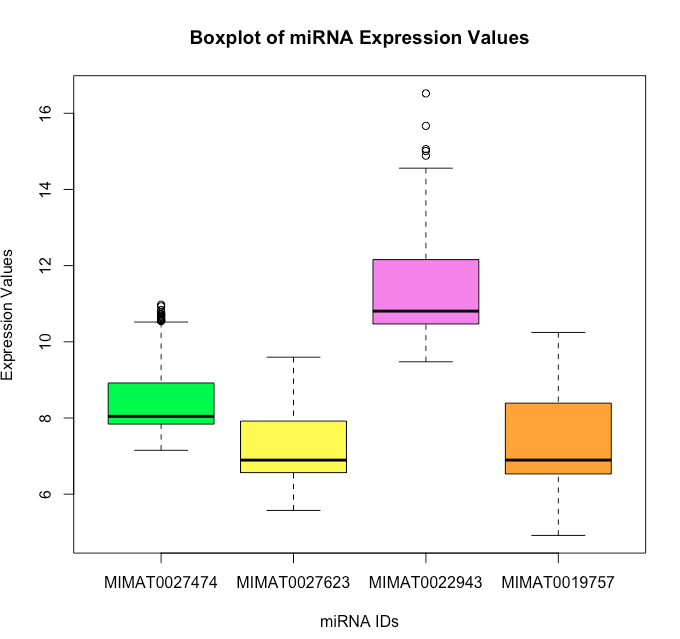
\includegraphics[scale=0.40]{Boxplot1.png}
\caption{Boxplot of Micro RNA Expression Values}
\label{fig:Boxplot1}
\end{figure}

\begin{figure}[htbp]
\centering
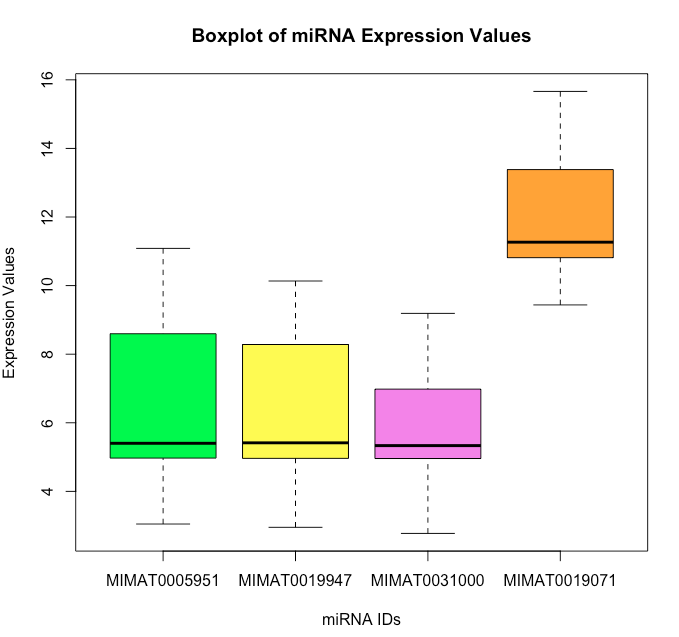
\includegraphics[scale=0.40]{Boxplot2.png}
\caption{Boxplot of Micro RNA Expression Values}
\label{fig:Boxplot2}
\end{figure}

\begin{figure}[htbp]
\centering
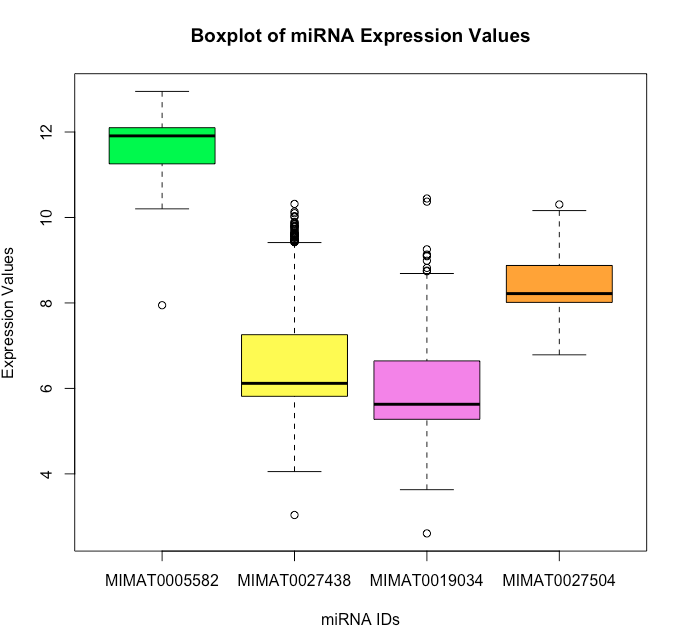
\includegraphics[scale=0.40]{Boxplot3.png}
\caption{Boxplot of Micro RNA Expression Values}
\label{fig:Boxplot3}
\end{figure}

\begin{figure}[htbp]
\centering
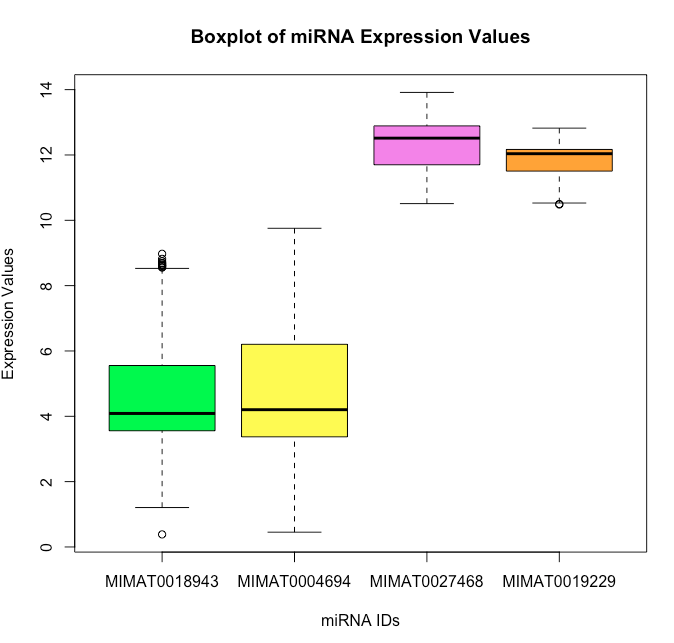
\includegraphics[scale=0.40]{Boxplot4.png}
\caption{Boxplot of Micro RNA Expression Values}
\label{fig:Boxplot4}
\end{figure}


{\textbf {\emph{Differential Expression Analysis}}}

Differential Expression Analysis is used to select two or more groups, say, "control" and "test" groups, and compare the average difference in expression values between the groups by statistical means. An open source suite of libraries called "Bio-Conductor" \cite{geoquery} was employed to conduct a differential expression analysis for this study. The miRNAs were ordered by decreasing differential expression values and the top 20 candidates were used to build the model. The expression data structure returned by Bioconductor::getGEO was converted to a data frame in order to perform a logistic regression analysis on the data frame using the candidate miRNA expression values as predictor variables. 


{\textbf {\emph{Training and Test Data}}}

The dataset was divided into a test set and training set. 65\% of the records were used to train the model and 35\% of the records was used for testing the model for prediction accuracy.


{\textbf {\emph{The Model}}}

Since the dependent variable was a boolean variable (diagnosis is either 1 or 0, representing whether the individual has breast cancer or not, respectively), a logistic regression approach was considered for modeling. A binary logistic regression is a method used to model data with a dichotomous dependent variable, or a binary outcome. Logistic regression can be mathematically expressed as in the equation \ref{eqn:logit}:

\begin{equation}
\label{eqn:logit}
    \ln(\frac{p}{(1-p)}) = a + \beta * X + e
\end{equation}

There were 20 candidate microRNAs chosen to be examined to determine which of them were potentially significant. The expression values were visually validated using Box plots. No missing values or outliers were observed. 

In the next step, a multivariate logistic regression model with all the significant variables was tried out for accuracy. The 'stat' library of R provides out of the box functions to run logistic regression as well as predict outcomes based on the model created. The function 'glm' (Generalized Linear Model) with an option to use binomial method, would conveniently return the logistic model. Using this, a multivariate logistic regression was performed with “diagnosis” as the dependent variable and the candidate miRNAs as the predictors.


The 'predict' method of the stat library returns the predicted values. By comparing the predicted outcomes with the actual outcomes in the test dataset, one can determine the accuracy of the model.  Various statistical methods were utilized to determine the predictive accuracy of the model.

{\it The p Value}

The 'p' values were analyzed for each of the predictor variables to evaluate their significance. The 'p' values were reported to have low values as expected for many of the predictor variables.

{\textbf {\emph{Model Benchmarking}}}

There were a number of methods to compare the accuracy of the models with one another. Using Accuracy, RMSE (Root Mean Square Error), Concordance vs Discordance ratio, misclassfication error, confusion matrix, Specificity vs Sensitivity, ROC curve and KS Plot the models were compared and classified based on their performance. Each of these methods helped in determination of the better model. 

{\it Overfitting and Underfitting}

The model prediction accuracy was assessed on the training data set and testing data set independently and found that there was no significant overfitting nor underfitting. 

{\it Accuracy}

Prediction error was calculated by taking the mean of all the differences between predicted outcomes and actual outcomes. Accuracy was measured using Equation \ref{eqn:AccuracyEqn}.

\begin{equation}
\label{eqn:AccuracyEqn}
    PredictionAccuracy = 1 - PredictionError
\end{equation}


{\it RMSE}

RMSE is a measure of how accurate the model is by squaring the differences of predictions and actuals and then taking the square root of their average. Lower the RMSE the better the model is. The equation \ref{eqn:RMSE} shows how to calculate RMSE. 

\begin{equation}
\label{eqn:RMSE}
RMSE = \sqrt{\frac{1}{n}\Sigma_{i=1}^{n}{\Big(\frac{d_i -f_i}{\sigma_i}\Big)^2}}
\end{equation}

{\it Confusion Matrix}

Confusion matrix gives a simple but useful interpretation of the model's accuracy. It gives a grid of true positives, false positives, true negatives and false negatives. This gives an idea where the model performs well and where it doesn't. From the library {\it InformationValue} the function {\it confusionMatrix()} was used to calculate the Confusion Matrix of the models that were studied.

{\it Kolmogorov-Smirnov Plot}

Kolmogorov-Smirnov test can be used for determining the performance of classification models. It tests the degree of separation between the positive and negative distributions in the models predicted output. From the library {\it InformationValue} the function {\it ks\_plot()} was used to plot the results of K-S chart.

\end{methods}

% \begin{figure}[!tpb]%figure1
% %\centerline{\includegraphics{fig01.eps}}
% \caption{Caption, caption.}\label{fig:01}
% \end{figure}

% \begin{figure}[!tpb]%figure2
% %\centerline{\includegraphics{fig02.eps}}
% \caption{Caption, caption.}\label{fig:02}
% \end{figure}

\section{Results and Discussion}

In this study, the GSE data was imported and a differential expression analysis was conducted using Bioconductor libraries. Of the top 250 miRNAs which found to be of statistical significance, 20 miRNAs were picked and used in a logistic regression model. 

{\it Differential Expression Analysis}

Using GEOQuery and limma libraries, a contrast matrix was formed and the top 250 miRNAs were selected, that have the most differential in their expression values in the microarray data. The top 25 of those miRNAs and corresponding differential values are given in figure \ref{fig:TopTable}.



{\it The Model Performance}

Various statistical methods were employed to determine the quality and accuracy of the model. The model demonstrated impressive results on all of these measured metrics. The summary of the results are given in table \ref{tab:modelperf}.

\begin{table}[htb]
\centering
\caption{Model Performance Metrics}
\label{tab:modelperf}
\begin{tabular}{ll}
\hline
\textbf{Model Performance Attribute} & \textbf{Value} \\ \hline
AIC Score                            & 255.49         \\
Accuracy                             & 97.9\%         \\
RMSE                                 & 0.128          \\
Concordance                          & 0.946          \\
Discordance                          & 0.054          \\
Misclassification Error              & 0.021          \\
Specificity                          & 0.992          \\ \hline
\end{tabular}
\end{table}



\begin{figure}[htbp]
\centering
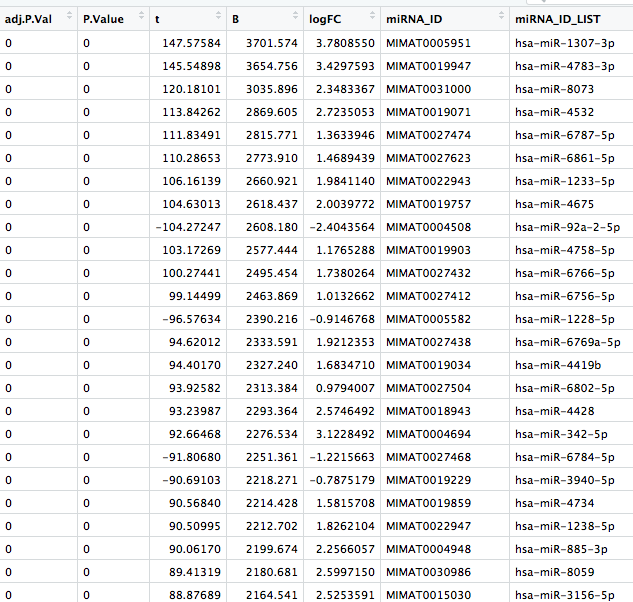
\includegraphics[scale=0.40]{TopTable.png}
\caption{TopTable of 250 miRNAs (Partial Listing)}
\label{fig:TopTable}
\end{figure}




{\it Model Summary}

The model summary below shows that there are many miRNAs, which play significant roles in predicting the chance of breast cancer. 



\begin{lstlisting}[label=LogisticModel, basicstyle=\tiny, caption=Model Summary, frame=htb]
> summary(model1)

Call:
glm(formula = fmla, family = binomial(), data = df_train, maxit = 100)

Deviance Residuals:
    Min       1Q   Median       3Q      Max
-3.6260  -0.0777  -0.0279   0.0002   3.0493

Coefficients:
               Estimate Std. Error z value Pr(>|z|)
(Intercept)  -118.77378   19.11571  -6.213 5.18e-10 ***
MIMAT0005951    0.63117    0.48151   1.311 0.189915
MIMAT0019947    0.66547    0.44339   1.501 0.133390
MIMAT0031000    1.71194    0.47502   3.604 0.000313 ***
MIMAT0019071    0.71815    0.47667   1.507 0.131914
MIMAT0027474    5.13266    0.91267   5.624 1.87e-08 ***
MIMAT0027623   -0.15988    0.83368  -0.192 0.847918
MIMAT0022943    1.97557    0.54316   3.637 0.000276 ***
MIMAT0019757   -1.91581    0.75942  -2.523 0.011645 *
MIMAT0004508   -0.17973    0.46236  -0.389 0.697477
MIMAT0019903    1.81081    1.20399   1.504 0.132579
MIMAT0027432    1.89852    0.65127   2.915 0.003556 **
MIMAT0027412   -0.22810    0.80367  -0.284 0.776542
MIMAT0005582    1.22016    0.90586   1.347 0.177995
MIMAT0027438   -0.96298    0.57017  -1.689 0.091232 .
MIMAT0019034   -0.05811    0.62558  -0.093 0.925990
MIMAT0027504    2.75982    0.97204   2.839 0.004522 **
MIMAT0018943    0.58781    0.37290   1.576 0.114955
MIMAT0004694   -1.48290    0.28678  -5.171 2.33e-07 ***
MIMAT0027468   -0.02877    0.78124  -0.037 0.970621
MIMAT0019229   -0.57278    0.97028  -0.590 0.554971
---
Signif. codes:  0 ‘***’ 0.001 ‘**’ 0.01 ‘*’ 0.05 ‘.’ 0.1 ‘ ’ 1

(Dispersion parameter for binomial family taken to be 1)

    Null deviance: 3155.69  on 2513  degrees of freedom
Residual deviance:  213.49  on 2493  degrees of freedom
AIC: 255.49

Number of Fisher Scoring iterations: 10
\end{lstlisting}


{\it Confusion Matrix}

The confusion matrix (table \ref{tab:conf-matrix}) shows that the model predicts the outcome with impressive accuracy. It mis-predicted 7 benign cases as breast cancer and 21 breast cancer cases as benign. It predicted 1326 cases accurately.


% Please add the following required packages to your document preamble:
% \usepackage{booktabs}
\begin{table}[htb]
\centering
\caption{}
\label{tab:conf-matrix}
\begin{tabular}{@{}ccc@{}}
\toprule
\textbf{Predicted}                  & \multicolumn{2}{c}{\textbf{Actual}}                                   \\ \midrule
\textit{\textbf{}}                  & \textit{\textbf{0 (No cancer)}} & \textit{\textbf{1 (Breast cancer)}} \\
\textit{\textbf{0 (No cancer)}}     & 895                             & 21                                  \\
\textit{\textbf{1 (Breast cancer)}} & 7                               & 431                                 \\ \bottomrule
\end{tabular}
\end{table}


{\it AUROC and Kolmogorov-Smirnov Test}

The selected model was studied further for more benchmarking methods such as plotting ROC curve as well as Kolmogorov–Smirnov plots (KS Plot). ROC curve shows 99.24\% of area under the curve. The ROC Plot (Figure \ref{fig:AUROC}) shows that the model has very good predictive abilities. Additionally the KS Plot (Figure \ref{fig:KSPlot}) shows that the model can predict much better than the random prediction at the mean level. 



\begin{figure}[htbp]
\centering
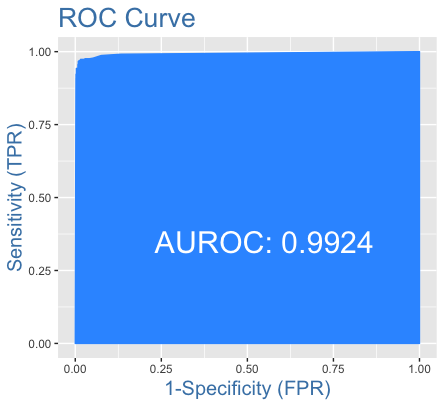
\includegraphics[scale=0.55]{ROC-Plot.png}
\caption{AUROC Plot}
\label{fig:AUROC}
\end{figure}

\begin{figure}[htbp]
\centering
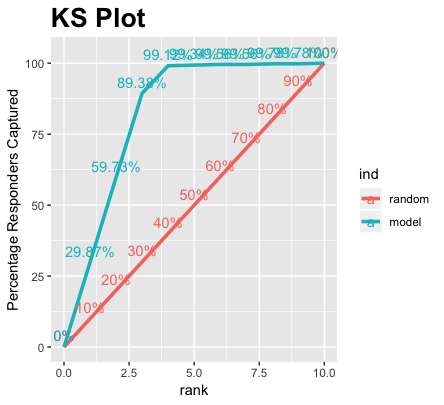
\includegraphics[scale=0.55]{KS-Plot.png}
\caption{KS Plot of the Model}
\label{fig:KSPlot}
\end{figure}


\section{Conclusion}

There were a number of findings from this study that were of significance.  A model with 20 predictor variables was found to be having very good predictive ability.
\begin{enumerate}
  \item MicroRNA expression values have notable predictive capability. 

  \item In practical terms, by using microRNA expression patterns in a patient, physicians can adequately identify a patient as at risk for developing breast cancer through the extent of expression in select microRNAs, and thereafter plan precautionary medical intervention. 

  \item The model accuracy could be improved by having more observations in the underlying data for the model to train and evaluate. Collecting more data from physicians would potentially improve the statistical significance of the findings of this study as well.

  \item Furthermore, the data should be adjusted according to the slight multicollinearity between independent variables as was observed in this study. This  would  eliminate  any  data  skewness  that  might  limit  the model’s predictive capabilities.
  \item Logistic regression is one of the widely used methods of modeling and prediction. Other machine learning, deep learning, and neural network approaches could further improve the predictive accuracy and reliability.  Newer algorithms and more cleaner data could assist physicians and other medical professionals to diagnose patients. 
\end{enumerate}

This analysis only scratched the surface of the untapped potential of using computational methods to detect cancer.  The power  and  promise  of  computational  sciences  with  larger  and  better  quality  data  could  be best utilized for improving healthcare and saving human lives.




\section*{Acknowledgement}
The author thanks Mr. Robert Gotwals for giving an opportunity and assistance to work on this interesting problem, as part of the NCSSM coursework, “Bioinformatics/Computational Biology", which in itself introduced the class a wide variety of tools and practices that immensely helped to conduct this study.  Appreciation is also extended to the NCSSM (North Carolina School of Science and Mathematics) for facilitating various computational sciences courses as part of the curriculum. The author is also grateful to NCBI, GEO for making this dataset publicly available for the use of researchers as well as the creators of Bioconductor libraries, which was adopted to conduct the Differential Expression Analysis.


%\bibliographystyle{natbib}
%\bibliographystyle{achemnat}
%\bibliographystyle{plainnat}
%\bibliographystyle{abbrv}
%\bibliographystyle{bioinformatics}
%
%\bibliographystyle{plain}
%
%\bibliography{Document}


\begin{thebibliography}{}
\bibitem{shimomura} Shimomura, A., Shiino, S., Kawauchi, J., Takizawa, S., Sakamoto, H., Matsuzaki, J., … Ochiya, T. (2016). Novel combination of serum microRNA for detecting breast cancer in the early stage. Cancer science, 107(3), 326–334. doi:10.1111/cas.12880

\bibitem{breast-cancer} How Common Is Breast Cancer? Retrieved from https://www.cancer.org/cancer/breast-cancer/about/how-common-is-breast-cancer.html

\bibitem{hormone-therapy} Hormone therapy for breast cancer. (2019, February 05). 
Retrieved from https://www.mayoclinic.org/tests-procedures/hormone-therapy-for-breast-cancer/about/pac-20384943


\bibitem{silveri} MicroRNA involvement in mammary gland development and breast cancer
Licia Silveri, Gaëlle Tilly, Jean-Luc Vilotte, Fabienne Le Provost
Reprod. Nutr. Dev. 46 (5) 549-556 (2006)
DOI: 10.1051/rnd:2006026
https://www.ncbi.nlm.nih.gov/pubmed/17107644/

\bibitem{brca} BRCA Mutations: Cancer Risk and Genetic Testing Retrieved from https://www.cancer.gov/about-cancer/causes-prevention/genetics/brca-fact-sheet



\bibitem{bartel} Bartel DP (January 2004). "MicroRNAs: genomics, biogenesis, mechanism, and function". 

Cell. 116 (2): 281–97. doi:10.1016/S0092-8674(04)00045-5. PMID 14744438.: 
https://www.ncbi.nlm.nih.gov/pubmed/14744438


\bibitem{microarray} DNA Microarray Technology Fact Sheet. (n.d.). Retrieved from https://www.genome.gov/about-genomics/fact-sheets/DNA-Microarray-Technology

\bibitem{ncbi-geo} GEO Overview  Retrieved from https://www.ncbi.nlm.nih.gov/geo/info/overview.html

\bibitem{geoquery} GEOquery. (n.d.). Retrieved from http://bioconductor.org/packages/release/bioc/html/GEOquery.html

\end{thebibliography}


\section{supplemental}


{\it Source Code}
\begin{verbatim}
#
# Import the libraries and clean up 
# the environment
#
library(Biobase)
library(GEOquery)
library(limma)
library(Metrics)
library(InformationValue)
library(car)

rm(list=ls())

#
# load series and platform data from GEO
#


gset <- getGEO("GSE73002", GSEMatrix =TRUE, 
            AnnotGPL=FALSE)

if (length(gset) > 1) {
    idx <- grep("GPL18941", 
        attr(gset, "names"))
} else { 
    idx <- 1
}

gset <- gset[[idx]]

#
# make proper column names to match toptable 
fvarLabels(gset) <- make.names(fvarLabels(gset))

# Seperating all diagnosises as breast cancer 
# and control
YY <- ifelse(gset$diagnosis == 
        "breast cancer", "1", 
        ifelse(gset$diagnosis == "non-cancer", 
        "0", "X"))

sel <- which(YY != "X")
gset <- gset[ ,sel]

#
# group names for all samples
masks <- ifelse(gset$diagnosis == "breast cancer", 
                "G1", "G0")


# log2 transform
ex <- exprs(gset)
qx <- as.numeric(quantile(ex, 
        c(0., 0.25, 0.5, 0.75, 0.99, 1.0), 
        na.rm=T))
LogC <- (qx[5] > 100) ||
  (qx[6]-qx[1] > 50 && qx[2] > 0) ||
  (qx[2] > 0 && qx[2] < 1 && qx[4] > 1 && 
  qx[4] < 2)
if (LogC) { ex[which(ex <= 0)] <- NaN
exprs(gset) <- log2(ex) }

#
# set up the data and proceed with analysis
fl <- as.factor(masks)
gset$description <- fl
design <- model.matrix(~ description + 0, gset)
colnames(design) <- levels(fl)
fit <- lmFit(gset, design)
cont.matrix <- makeContrasts(G1-G0, 
        levels=design)
fit2 <- contrasts.fit(fit, cont.matrix)
fit2 <- eBayes(fit2, 0.01)
tT <- topTable(fit2, adjust="fdr", 
        sort.by="B", number=250)


# Final Top Table of 250
tT <- subset(tT, 
        select=c("ID","adj.P.Val","P.Value",
            "t","B","logFC", "miRNA_ID",
            "miRNA_ID_LIST"))
write.table(tT, file=stdout(), 
        row.names=F, sep="\t")


dataframe1 <- data.frame(gset) 
Y <- ifelse(gset$`diagnosis:ch1` == 
            "breast cancer", 1, 0)
dataframe1$Y <- Y
miRNAIDs <- tT$ID[1:100]
final_dataframe <- subset(dataframe1, 
        select=c(miRNAIDs, "Y"))
final_dataframe <- na.omit(final_dataframe)

#
# Create model formula

idx <- 20
fmla <- paste("Y~")
for (var1 in miRNAIDs[1:idx]) {
  
  fmla <- paste(fmla, var1, sep = "") 
  if (var1 != miRNAIDs[idx])
    fmla <- paste(fmla, "+", sep = "")
}

#
# Create the final data frame with all data 

final_dataframe <- 
    final_dataframe[sample(nrow(
                final_dataframe)),]
#
# Boxplots of selected miRNAs
#
for (i in c(1, 5, 13, 17)) {
  print (i)
  print(miRNAIDs[i:i+3])
  boxplot(subset(final_dataframe, 
    select=c(miRNAIDs[i:(i+3)])), 
    main="Boxplot of miRNA Expression Values", 
    xlab="miRNA IDs", ylab="Expression Values",
    col=c("green", "yellow", 
        "violet", "orange"))
}


#
# Set seed to ensure the model 
# may be replicated. 

set.seed(143)

#
# Split the data frame into training 
# and testing data sets. 

sample_size <- 
    floor(0.65*(nrow(final_dataframe)))
my_flag <- 
    sample(seq_len(nrow(final_dataframe)), 
        size = sample_size)
df_train <- final_dataframe[my_flag, ]
df_test <- final_dataframe[-my_flag, ]

nrow(df_train)
nrow(df_test)

#
# Build the model 

model1 <- glm(fmla, family=binomial(), 
            data = df_train, maxit = 100)
summary(model1)


#
# Prediction and Error Analysis

prediction1 <- predict(model1, newdata = df_test, 
                    type = "response")
fitted_results <- ifelse(prediction1 > 0.5, 1, 0)
prediction_error <- mean(fitted_results 
                            != df_test$Y)

#
# Statistical analyses
#
rmsescore <- rmse(prediction1, df_test$Y)

print(paste("Formula: ", mla)
print(summary(model1))
print(paste("ACCURACY:", 1-prediction_error))
print(paste("RMSE:", rmsescore) )
print("Concordance Analysis:")
print(Concordance(df_test$Y, fitted_results))
print("Misclassification Error Analysis:")
print(misClassError(df_test$Y, fitted_results))
print("Specificity Analysis:")
print(specificity(df_test$Y, fitted_results))
print("Confusion Matrix:")
print(confusionMatrix(df_test$Y, 
            fitted_results))
sensMatrix <- plotROC(df_test$Y, 
        prediction1, Show.labels = F, 
        returnSensitivityMat = T)
ks_plot(df_test$Y, prediction1)

#
# This is a VIF model. A VIF score is generated 
# to figure out multicollinearity using the VIF 
# score. All VIF scores greater than 2.5 could 
# be significant concerning. 
#
vif(model1)

\end{verbatim}


\end{document}
